\documentclass[11pt,a4paper]{article}
\usepackage[utf8]{inputenc}
\usepackage[T1]{fontenc}
\usepackage{amsfonts}
\usepackage[french]{babel}
\frenchbsetup{StandardLists=true} % à inclure si on utilise \usepackage[francais]{babel}
\usepackage{enumitem}
\usepackage{amssymb}
\usepackage{amsmath}
\usepackage[left=2cm,right=2cm,top=2cm,bottom=2cm]{geometry}
\usepackage{multirow}
\usepackage[dvipsnames]{xcolor}

\usepackage[T1]{fontenc}
\usepackage{fouriernc}
\usepackage{graphicx}

\usepackage{setspace}
\singlespacing

\usepackage{pstricks}
\usepackage{xkeyval}
\usepackage{pst-labo}


\usepackage{multicol}
\usepackage{caption}
\usepackage{fancyhdr}
\pagestyle{fancy}
\renewcommand\headrulewidth{1pt}
\fancyhead[L]{Lycée Denis Diderot }
\fancyhead[R]{Classe de 1 Bac Pro }
\setcounter{page}{8}\fancyfoot[C]{page \thepage}
\fancyfoot[R]{Année 2024-2025}
\fancyfoot[L]{Alexis RUIZ}
\usepackage{multirow,tabularx,booktabs}
\newcommand{\cadreblanc}[1]{%
\medskip\framebox[\linewidth][c]{%
\rule{0mm}{#1mm}}\par
\medskip}

\usepackage{awesomebox}
\setlength{\aweboxvskip}{0mm}
\usepackage{pifont}
\usepackage{chemmacros}
\chemsetup{modules=all}
\setlength{\columnseprule}{.25mm}

\renewcommand{\arraystretch}{2}
\newcolumntype{C}[1]{>{\centering\arraybackslash }b{#1}}

\newcommand*\acocher{\quitvmode{\fboxsep0pt \fboxrule0.8pt \fbox{\vrule height1.8ex depth.1ex width0pt \vrule height0pt depth0pt width1.9ex }}}

\newcommand{\code}{\awesomebox[black]{2pt}{

\includegraphics[scale=0.15]{images/frame.png}
}{black}}

\newcommand{\moteur}{\awesomebox[black]{2pt}{

\includegraphics[scale=1]{images/moteur.jpg} 
}{black}}

\newcommand{\defconclusion}{\awesomebox[black]{2pt}{\rotatebox{90}{\Large{\textbf{Conclusion}}}}{black}}

\usepackage[tikz]{bclogo} 
\newcommand{\ctext}[1]
{\begin{bclogo}[couleur = white,logo= , arrondi = 0.1,barre=none]
{}
\vspace{-8mm}
~~
\textcolor{red}{#1}
~~
\end{bclogo}}



  \newenvironment{itemize*}%  % listes compactes
    {\begin{itemize}%
      \setlength{\itemsep}{0pt}%
      \setlength{\parskip}{0pt}}%
    {\end{itemize}}


\frenchbsetup{StandardLists=true}



\begin{document}


\begin{center}
 \LARGE{COURS } \\[3mm]
\end{center}



\normalsize

\hrule\
\\[0,1cm]


\fcolorbox{black}{white}{\textbf{\ding{202} Puissance électrique en régime continu}}\\
\vspace{-3mm}
\begin{itemize*}
\item \textbf{Puissance électrique reçue par un appareil en régime continu} 
\noindent% 

\begin{minipage}{.67\textwidth}%
 \ctext{La \textbf{puissance électrique P} (en watt) reçue par un appareil soumis à une tension continue U (en volt) et traversée par un courant d'intensité I (en ampères) est donné par la relation :  }

\end{minipage}%
\hfill
\begin{minipage}{.25\textwidth}%
 \ctext{
     ~~~~~~\LARGE{$\mathrm{P = U\times I}$} \\[3mm]
     \hspace{1cm}\small{avec P(W), U(V) et I(A)} 
}
\end{minipage}%

\item \textbf{Puissance électrique reçue par un appareil en régime continu} \\ La puissance consommée par un appareil électrique se mesure avec un wattmètre ou avec un voltmètre en dérivation et un ampèremètre en série.

\noindent%
\hfill
\begin{minipage}{.20\textwidth}%

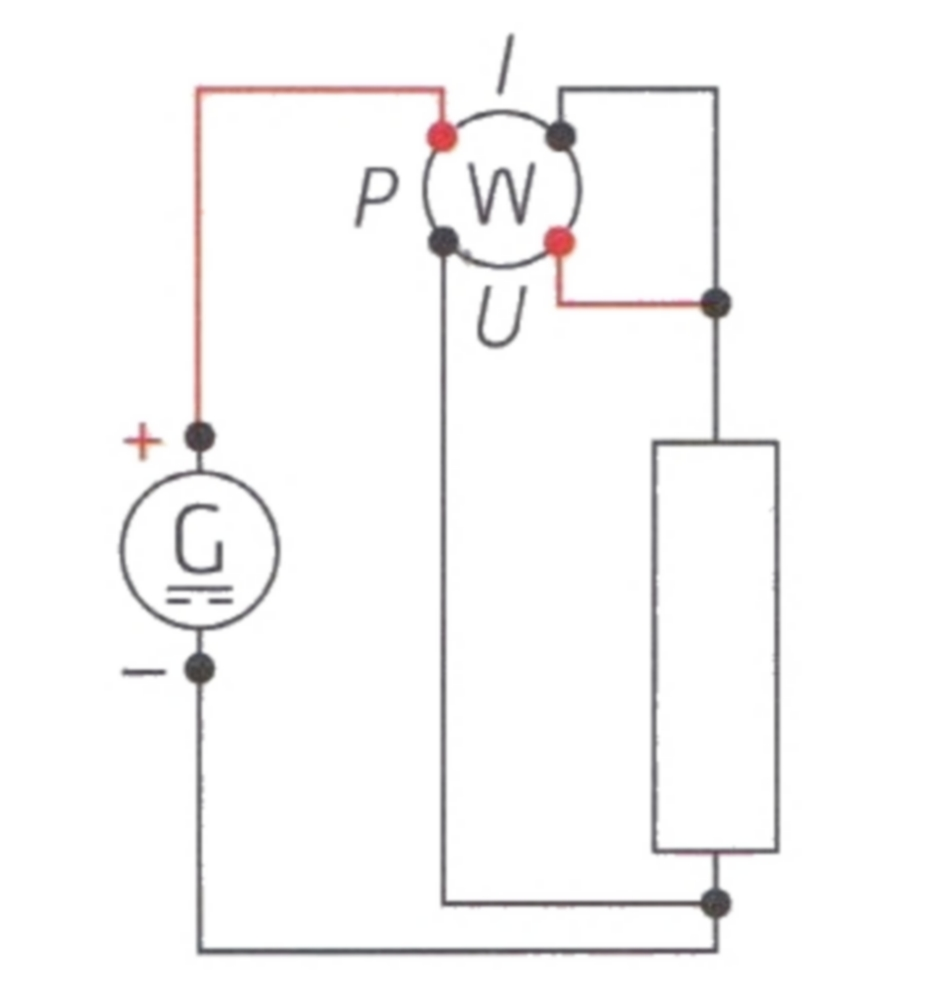
\includegraphics[width=\textwidth]{images/Cours - wattmetre.jpg}

\end{minipage}%
\hspace{3cm}
\begin{minipage}{.30\textwidth}%
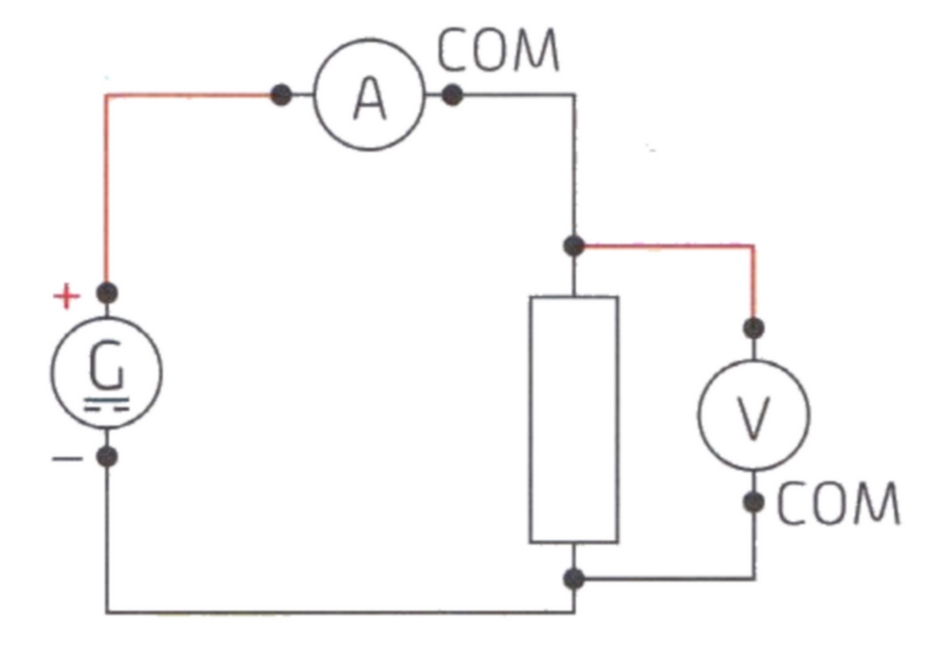
\includegraphics[width=\textwidth]{images/Cours - wattmetre2.jpg}
\end{minipage}%


\item \textbf{Valeurs nominales :} L'intensité nominale $I_N$, la tension nominale $U_N$  et la puissance nominale $P_N$ d'un récepteur correspondent aux valeurs de fonctionnement dans les conditions normales données par le fabricant. Elles sont inscrites sur la plaque signalétique ou la notice d'utilisation. 

\item \textbf{Puissance totale :} La puissance totale consommée par un ensemble d'appareils est égale à la somme des puissances reçues par ces appareils, qu'ils soient branchés en série et / ou en dérivation.  

\end{itemize*}

\fcolorbox{black}{white}{\textbf{\ding{203} Énergie électrique}}\\[-3mm]
\begin{itemize*}
    \item \textbf{Calcul de l'énergie électrique}\\
\noindent%
\begin{minipage}{.67\textwidth}%
    
    \ctext{En régime continu et en régime alternatif, l'énergie électrique E (en Joule) reçue par un appareil de puissance P (en watt) pendant une durée t (en seconde) est donné par la relation:}

\end{minipage}%
\hfill
\begin{minipage}{.25\textwidth}%
\ctext{
     ~~~~~~\LARGE{$\mathrm{E = P\times t}$} \\[3mm]
     \hspace{1cm}\small{avec E(J), P(W) et t(s)} 
}
\end{minipage}%





    \item \textbf{Mesure de l'énergie électrique}\\
    L'énergie électrique consommée par un appareil électrique se mesure avec \textbf{un compteur d'énergie} ou \textbf{un joulemètre}. 
    \item \textbf{Unités et coût}\\
    \vspace{-5mm}\begin{center}
    

    \begin{tabular}{|C{3cm}|C{4cm}|C{3cm}|C{3cm}|}
         \hline
        Grandeur & Énergie $E$ & Puissance $P$ & Temps $t$\\
         \hline
        Unité SI & \textcolor{red}{Joule (J)} & \textcolor{red}{Watt (W)} & \textcolor{red}{Seconde  (s)}  \\
         \hline
         Unité usuelle &  \textcolor{red}{kilowattheure (kWh)}&  \textcolor{red}{kilowatt (kW)}  &  \textcolor{red}{heure (h)}  \\
         \hline
        
    \end{tabular}
    
\vspace{2mm}
\ctext{
1 Wh = 1 W $\mathrm{\times 1~h = 1~W \times 3 600~s  = 3600~J }$ \\
1 kWh = 1 kW $\mathrm{\times 1~h = 1000~W \times 3 600~s  = 3~600~000~J = 3,6 \times 10^{6}~J = 3,6~MJ (megajoule)}$ \\
Une facture d'électricité est établie à partir de la consommation d'énergie électrique en kwh }
\end{center}

\end{itemize*}


\end{document}